\documentclass[conference]{IEEEtran}
\IEEEoverridecommandlockouts
% The preceding line is only needed to identify funding in the first footnote. If that is unneeded, please comment it out.
\usepackage{cite}
\usepackage{amsmath,amssymb,amsfonts}
\usepackage{algorithmic}
\usepackage{graphicx}
\usepackage{textcomp}
\usepackage{xcolor}
\usepackage{float}
\usepackage{ifthen}
\def\BibTeX{{\rm B\kern-.05em{\sc i\kern-.025em b}\kern-.08em
    T\kern-.1667em\lower.7ex\hbox{E}\kern-.125emX}}
\begin{document}

\title{Pump it Up: Data Mining the Water Table\\
{\footnotesize \textsuperscript{*}The prediction and characteristics of operating condition of waterpoints in Tanzania by using data modelling, analysis and machine learning}
}

\author{\IEEEauthorblockN{1\textsuperscript{st} Wenxuan Zhu}
\IEEEauthorblockA{\textit{University of Nottingham} \\
\textit{20379163}\\
Nottingham, UK \\
alywz30@nottingham.ac.uk}
\and
\IEEEauthorblockN{2\textsuperscript{nd} Hong Li}
\IEEEauthorblockA{\textit{University of Nottingham} \\
\textit{20438363}\\
Nottingham, UK \\
psxhl10@nottingham.ac.uk}
}

\maketitle

\begin{abstract}

    Pump it Up: Data Mining the Water Table is a dataset about the pump water supply system in Tanzania. In this paper, we use data analysis, data preprocessing, and data classification methods to analyze and process the dataset in detail, and develop Decision tree and XGBoost (eXtreme Gradient Boosting) models to analyze the correlation of data features and predict the operation status of water pumps. And the performance of the two models is compared. The research results show that XGBoost has good performance, with an accuracy of 84.1\%. In addition, we also conducted a comparative analysis of natural and human factors and studied their relationship with water point conditions. This has important reference value for decision-makers and water supply managers, which can help them better understand and optimize the operation of pump water supply system and ensure the supply of water resources.
    

\end{abstract}

\begin{IEEEkeywords}
data modelling, data analysis, machine learning
\end{IEEEkeywords}

\section{Introduction}

Providing clean and reliable water is crucial for community well-being and sustainable development. In many underdeveloped areas, obtaining safe water remains a challenge, with a significant number of water pumps and systems facing issues such as malfunction, breakdowns, and inadequate maintenance. In order to solve these problems, governments and societies in various countries have invested a large amount of manpower and material resources. An open source web app named Taarifa aggregated data from the Tanzania Ministry of Water and the Pump it Up: Data Mining the Water Table dataset was created to explore and analyze factors related to the functionality of Tanzania water pumps.

\subsection{Introduction to the data set}

The data set comes from the waterpoints dashboard of an open source web app named “Taarifa” which aggregates data from the Tanzania Ministry of Water. This data set aims to help predict and improve the operational status of water pumps in Tanzania, in order to provide reliable drinking water supply. 

The dataset is divided into a training set and a testing set, the training set has 59.4k instances and 41 attributes including the label that save in the a separate file, in the case of testing data has 14.85k instances. The data set contains a large amount of information about pumps and water supply systems, including geographical location, pump type, water source type, construction year, pump management and maintenance status, etc. These data features can be used to predict the functional status of water pumps, help decision-makers and water resource managers understand the operational status of water supply systems, and take corresponding measures to improve water supply services. The target variable of the study is status\_group that has three possible values functional, non-functional and functional needs repair. As shown in Figure 1, this is the label display diagram corresponding to the training set, which contains pumps in three states: functional, non-functional and functional needs repair.

\begin{figure}[htbp]
\centerline{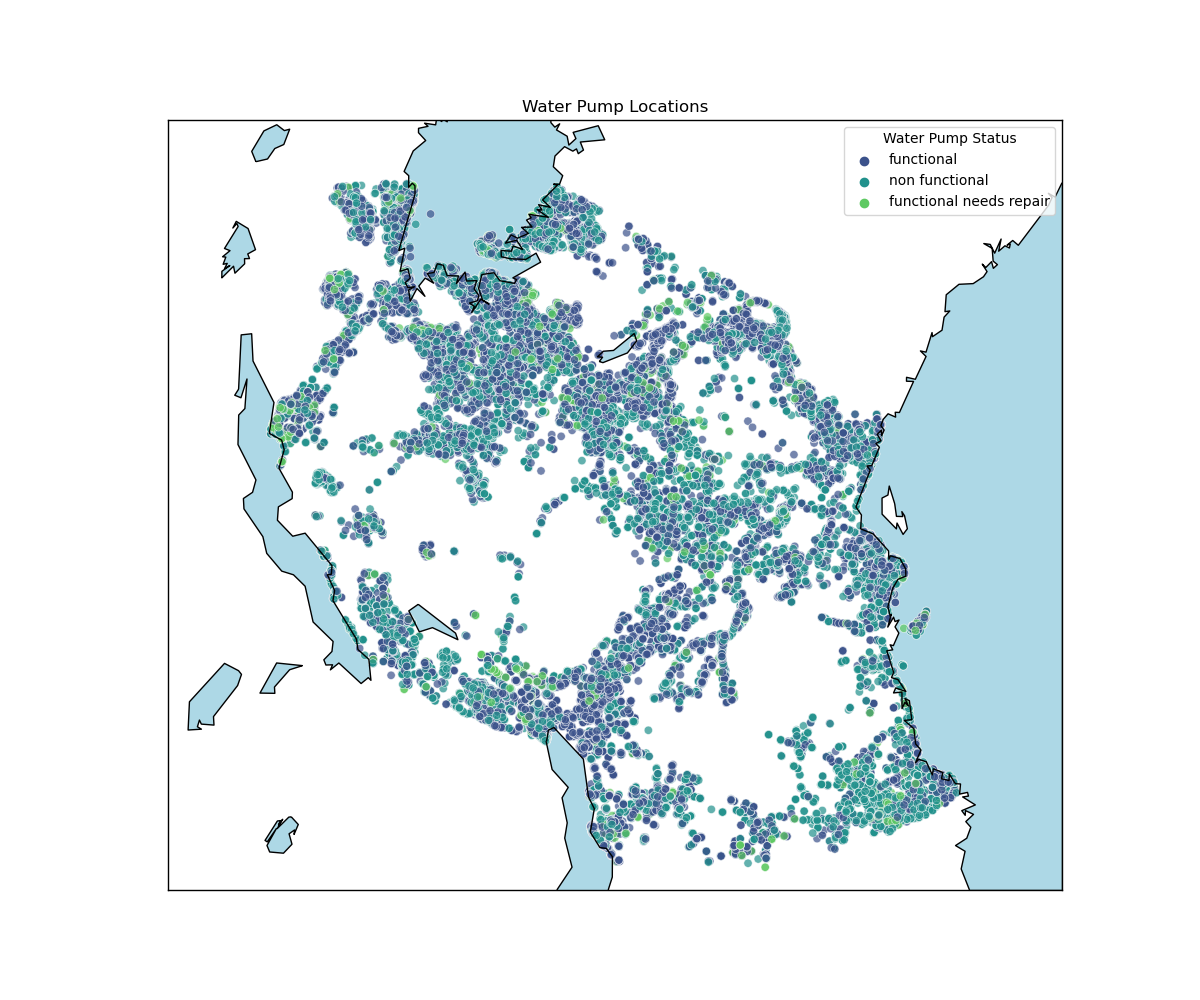
\includegraphics[width=0.5\textwidth]{introduction.pic.jpg}}
\caption{Water pump locations}
\end{figure}

\subsection{Research questions}

\subsubsection{How to predict the health of each recorded water point in the data set. (To improve maintenance operations and ensure cleanliness)}

\begin{itemize}
\item How to ensure that data is accurate, adequate and properly distributed.
\item How to judge the impact of features on forecast results and how to select them for prediction.
\item How to choose the right machine learning model for prediction.
\item How to judge the quality of forecast results.
\end{itemize}

\subsubsection{Whether natural factors (Like water quality, source type and so on) have more influence on the condition of a water-point or human factors (Like management). (For key decision maker to know they need to pay more attention on natural factors or human factors in the future)}

\begin{itemize}
\item Which features are natural factors.
\item Which features are human factors.
\item How to reflect the relationship between a class of eigenvalues and condition of a waterpoint.
\end{itemize}

In this article, we provide a detailed analysis of this dataset using several different data science and machine learning techniques. Our goal is to identify key characteristics and patterns to predict the function of water pumps to help managers better manage water resources. By understanding the factors that affect pump function, stakeholders can efficiently allocate resources, prioritize maintenance efforts, and ensure sustainable access to clean water for residents. In addition, we will also compare these data processing methods and the performance of models built using machine learning from different aspects, such as the prediction accuracy of training, etc.

The remainder of this paper is organized as follows. Section 2 outlines related work using this dataset for data mining and predicting water pump function. Section 3 introduces the methods we choose for data analysis, preprocessing and data classification and the corresponding results of each method. Section 4 focuses on discussing and comparing the results of different methods with the dataset research results of previous related work. Section 5 presents conclusions and suggestions for future research.

Overall, this paper aims to use a variety of data mining techniques to predict the condition of water supply points, understand the data characteristics that affect the function of water pumps, and provide decision support for key decision makers, so as to contribute to the development of sustainable water resource management strategies and policies.


\section{Literature Review}

Data mining technology is increasingly being applied in fields such as business and scientific research. It can be predicted and analyzed through historical data analysis and pattern recognition. Therefore, data mining technology has also been applied to water resource management to maximize the utilization of water resources on Earth and ensure the supply of water resources. The following are some studies on using data mining techniques to predict the condition of water pumps in Tanzania.

Darmatasia and Aniati \cite{b1} used XGBoost (eXtreme Gradient Boosting) data mining methods to analyze and predict the state of water pumps. At the same time, they also proposed using recursive feature elimination to select important data features to improve the accuracy of the model. They selected 27 optimal features from 39 features in the dataset to train and evaluate the model, and achieved an accuracy of 80.38\%.

Karan and L \cite{b2} utilize TabNet, a sequential attentive deep neural architecture, for predicting the repair status of water pumps in Tanzania. TabNet utilizes a sequence attention mechanism to model table data, extracting key features through feature selection and automatic learning processes. TabNet also provides model interpretability, explaining the predicted results of the model through attention weights and feature selection. They also use $\alpha$-Balanced variant of focal loss to address category imbalance issues.

Jacob \cite{b3} used classification tree and RandomForest algorithm to create different models, and implemented the all-in-one classification method. In addition, he also established multiple models such as logical regression and the boosted logistic regression for comparison and evaluation. The final result is that the RandomForest algorithm performs best in AUC (area under the curve) and classification rate, which are 0.91 and 0.8209 respectively, and the model can also help to understand why pumps are more likely to belong to a certain category and the relationship between variables.

Indra and Vivek \cite{b4} created several models by using SAS® Enterprise Miner, including decision trees, neural networks, multinomial logistic regression and random forest models, to classify and predict whether pumps are in functional state, non-functional state or in need of maintenance. They evaluate the performance of each model by verifying the misclassification rate, and the best model is the RandomForest model.

\section{Methodology and Results from each of the stages}

In order to carry out effective data mining and analysis on the data set, we started from three aspects: data analysis, data preprocessing and data classification, and we tried at least two methods in each aspect, and each method showed different results. Below, we will introduce the methodology and display the results from these three aspects.

\subsection{Data analysis}

In terms of data analysis, we used two analysis methods, namely descriptive statistical analysis and data visualization, by using these methods, we performed data analysis on the data set before and after data imputation.

\subsubsection{Descriptive statistical analysis (before data imputation)}

As shown in Fig. 2, first we use the .info command of pandas to count the general information of the original data set, which helps us to observe the features and feature types in the data set more intuitively.

\begin{figure}[htbp]
\centerline{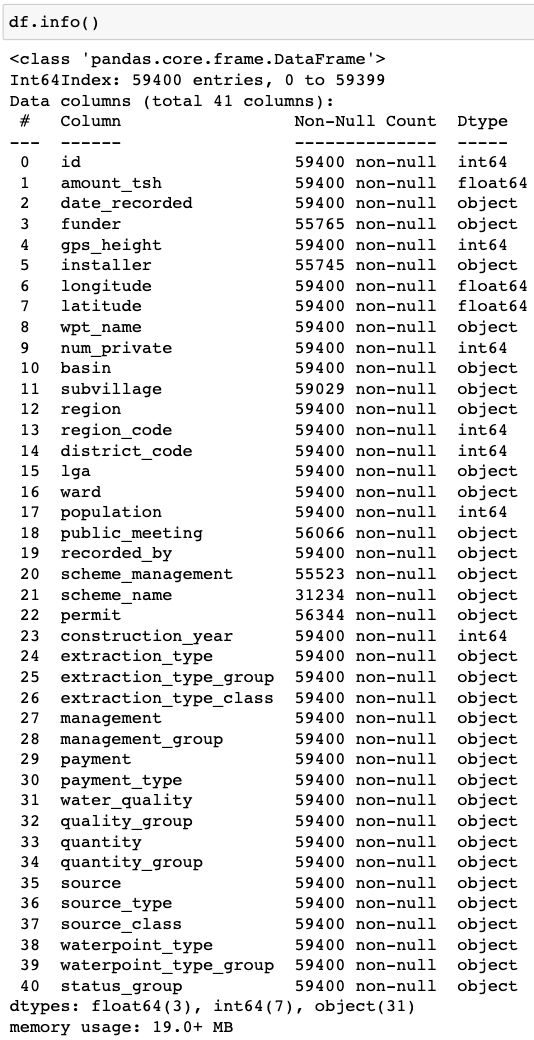
\includegraphics[width=0.3\textwidth]{1.pic.jpg}}
\caption{General information about the dataset}
\end{figure}

Second, as shown in Fig. 3, we distinguish all features according to their data types, which will benefit classification research for data visualization and subsequent data preprocessing.

\begin{figure}[htbp]
\centerline{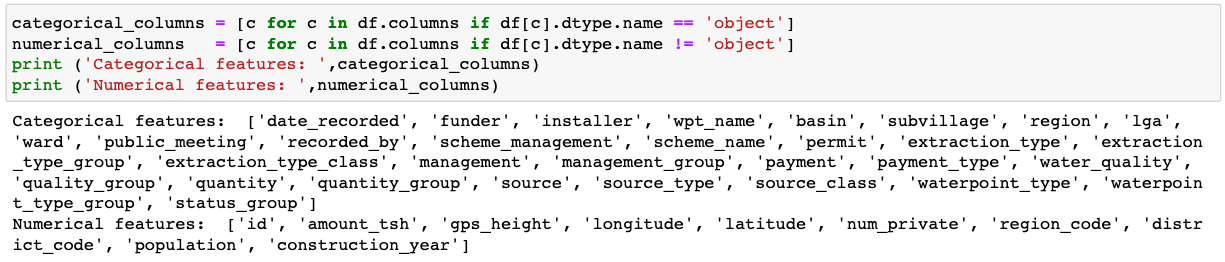
\includegraphics[width=0.5\textwidth]{2.pic.jpg}}
\caption{Feature types of the dataset}
\end{figure}

Finally, as shown in Fig. 4, we find out all the NaNs in the dataset and find their corresponding feature names.

\begin{figure}[H]
\centerline{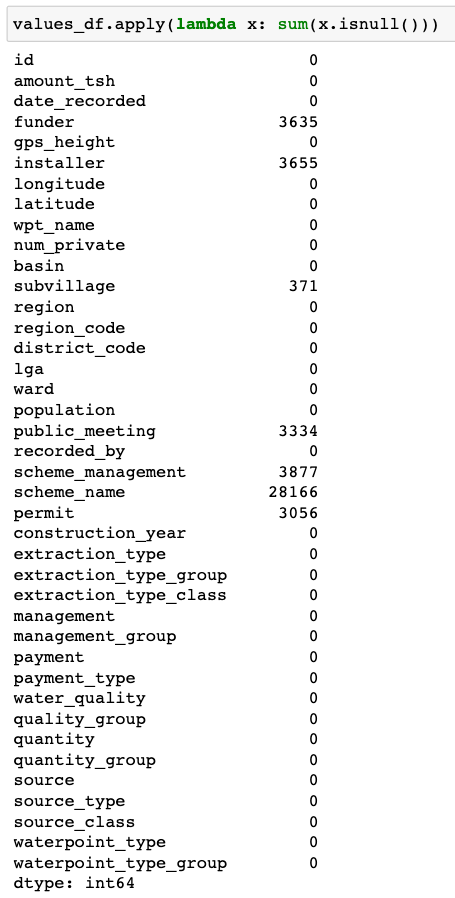
\includegraphics[width=0.2\textwidth]{3.pic.jpg}}
\caption{Check for NaNs}
\end{figure}

\subsubsection{Data visualization (before data imputation)}

Next, we perform visual analysis on some important features of the raw data.

\begin{figure}[H]
\centerline{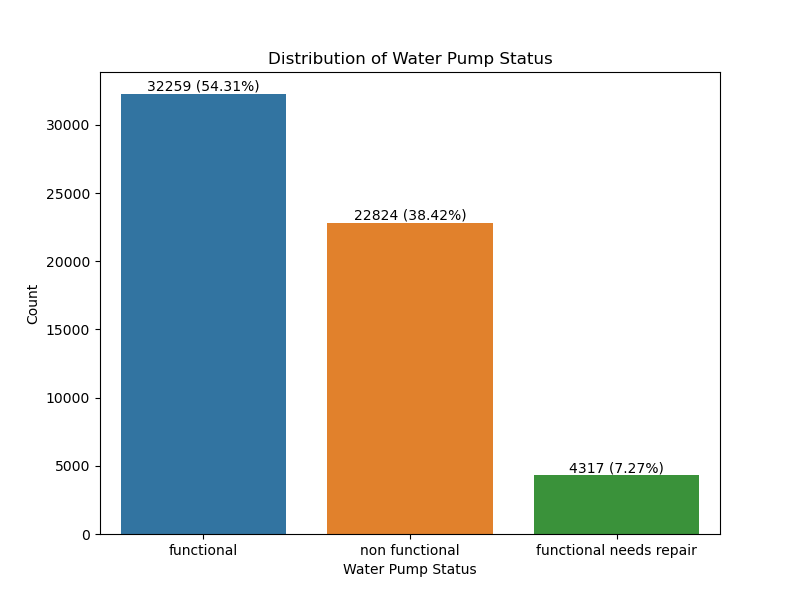
\includegraphics[width=0.5\textwidth]{4.pic.jpg}}
\caption{Distribution of water pump status}
\end{figure}

In Fig. 5, it can be clearly seen that functional and non functional water pumps account for the majority, with a total of 32259 functional water pumps accounting for 54.31\%, and 22824 non-functional water pumps accounting for 38.42\%. However, only a small portion of functional water pumps needs repair, with only 4317 pumps accounting for 7.27\%. This is a category imbalance situation that may lead to model bias during training and prediction. This may reduce the accuracy and recall rate of the model for rare categories. To solve this problem, we need to adopt some strategies, such as undersampling or oversampling, to balance the number of samples in each category.

\begin{figure}[H]
\centerline{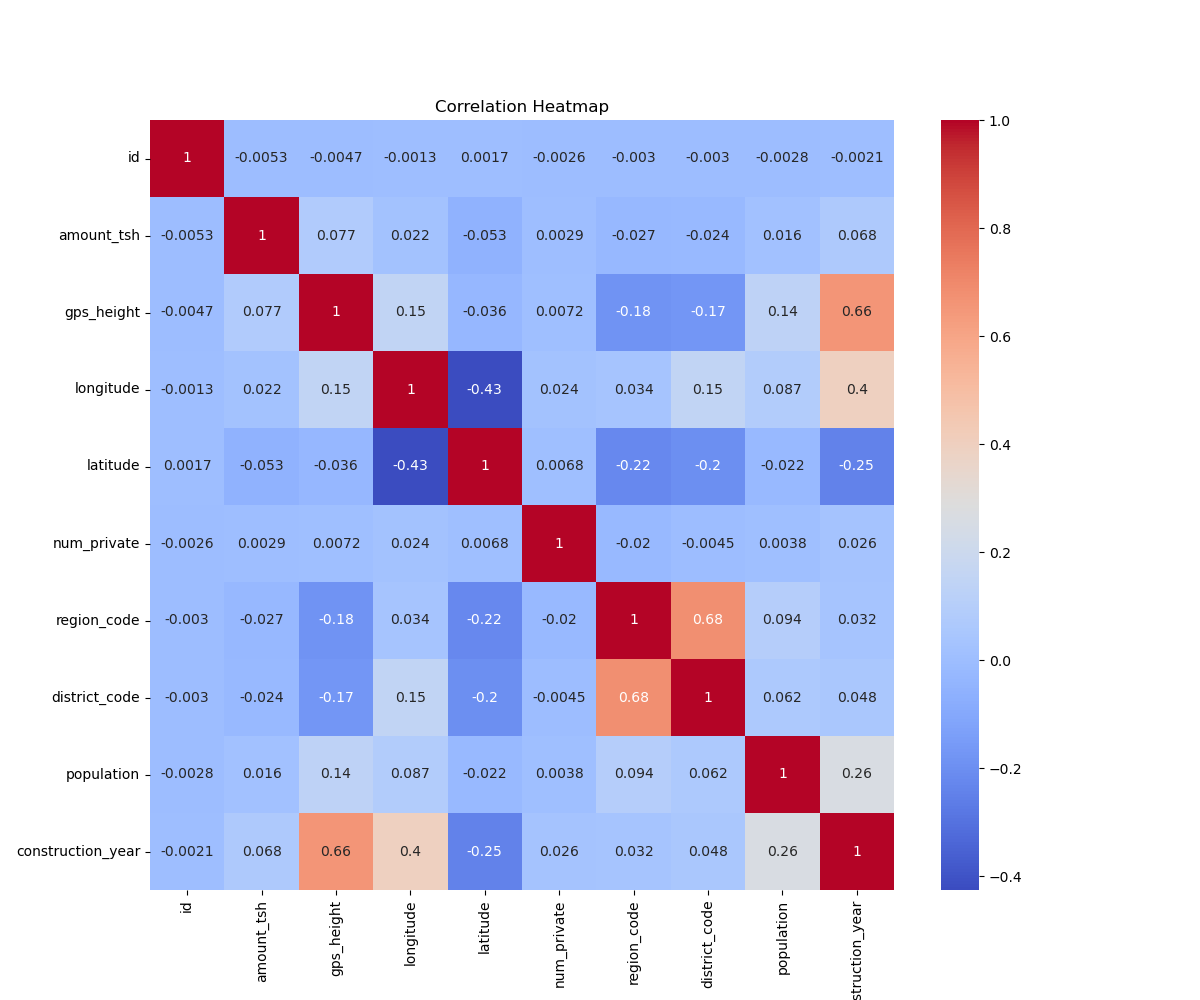
\includegraphics[width=0.5\textwidth]{5.pic.jpg}}
\caption{Correlation heatmap}
\end{figure}

From Fig. 6, it can be seen that the correlation between data features of numerical types, with darker colors indicating a high degree of correlation between features, such as GPS\_ height and construction\_ year, longitude and construction\_ year. At the same time, it should be noted that there may be multicollinearity between these highly correlated features, which may have an impact on the performance and interpretability of the model. Therefore, these data features need to be identified and further processed. In addition, some features may not have a significant correlation with the state of the water pump, which does not have a strong influence on predicting the state of the water pump. Therefore, these features may not be considered during training and testing.

\subsubsection{Data visualization (after data imputation)}

In view of the fact that some NaNs were found in descriptive statistics, and in order to find more data problems and analyze them, we slightly modified the data set, used the mode to imput NaNs, and conducted data analysis for research questions.

In order to study question 1, it is necessary to find which features are more relevant to the target features and select which ones are used for prediction. Therefore, after data interpolation, in order to visualize the characteristics of the object data type, it is necessary to visualize These features were encoded before so that they can be displayed more intuitively.

\begin{figure}[H]
\centerline{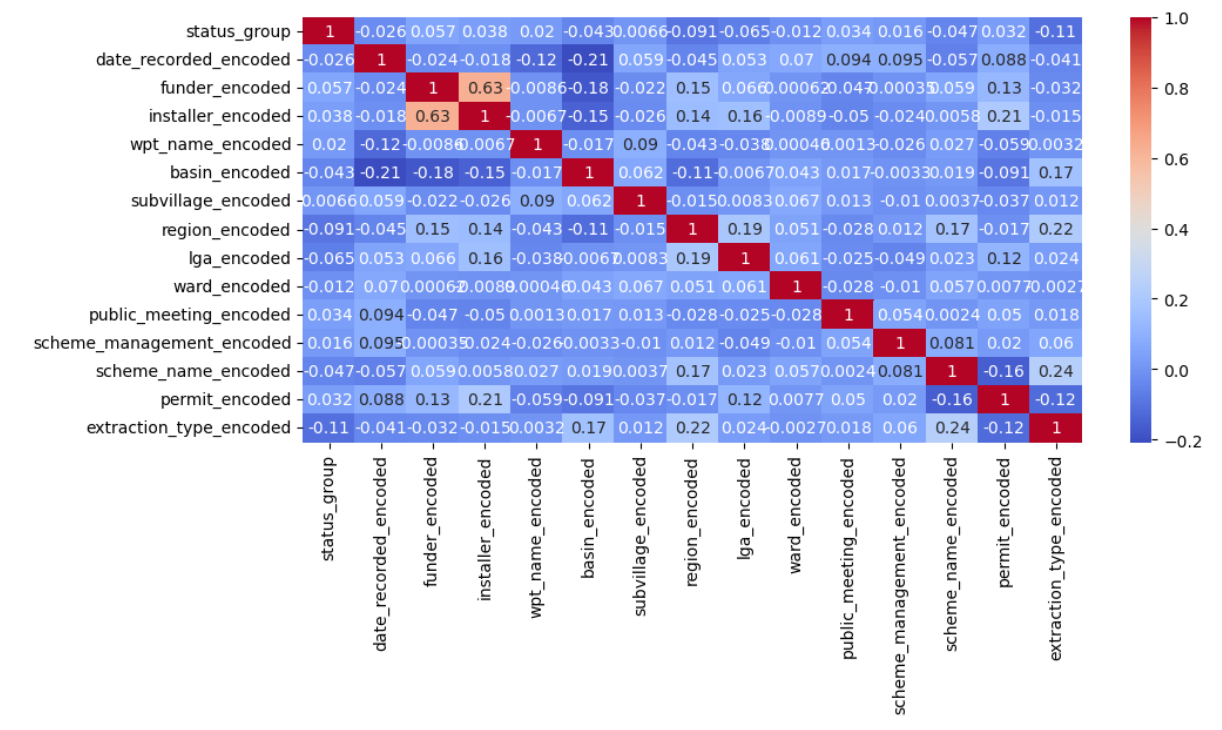
\includegraphics[width=0.5\textwidth]{6.pic.jpg}}
\caption{Heatmap for 'object' features}
\end{figure}
    
As shown in Fig. 7, the logic is the same as that in Fig. 6. The darker the color, the higher the correlation between the features. For example, there may be a higher correlation between 'extraction\_type' and the status of the water pump.

In order to analyze research question 2, we need to find out the characteristics of nature factors and human factors separately, and try to find out the connection between them through visualization. For example, if we choose 'water quality' as the nature factors and 'management' as the human factors, try to draw a stacked histogram. As shown in Fig. 8, it seems that the better the 'water quality', the more water pumps can be used, and the nature factors may have a greater impact.

\begin{figure}[H]
\centerline{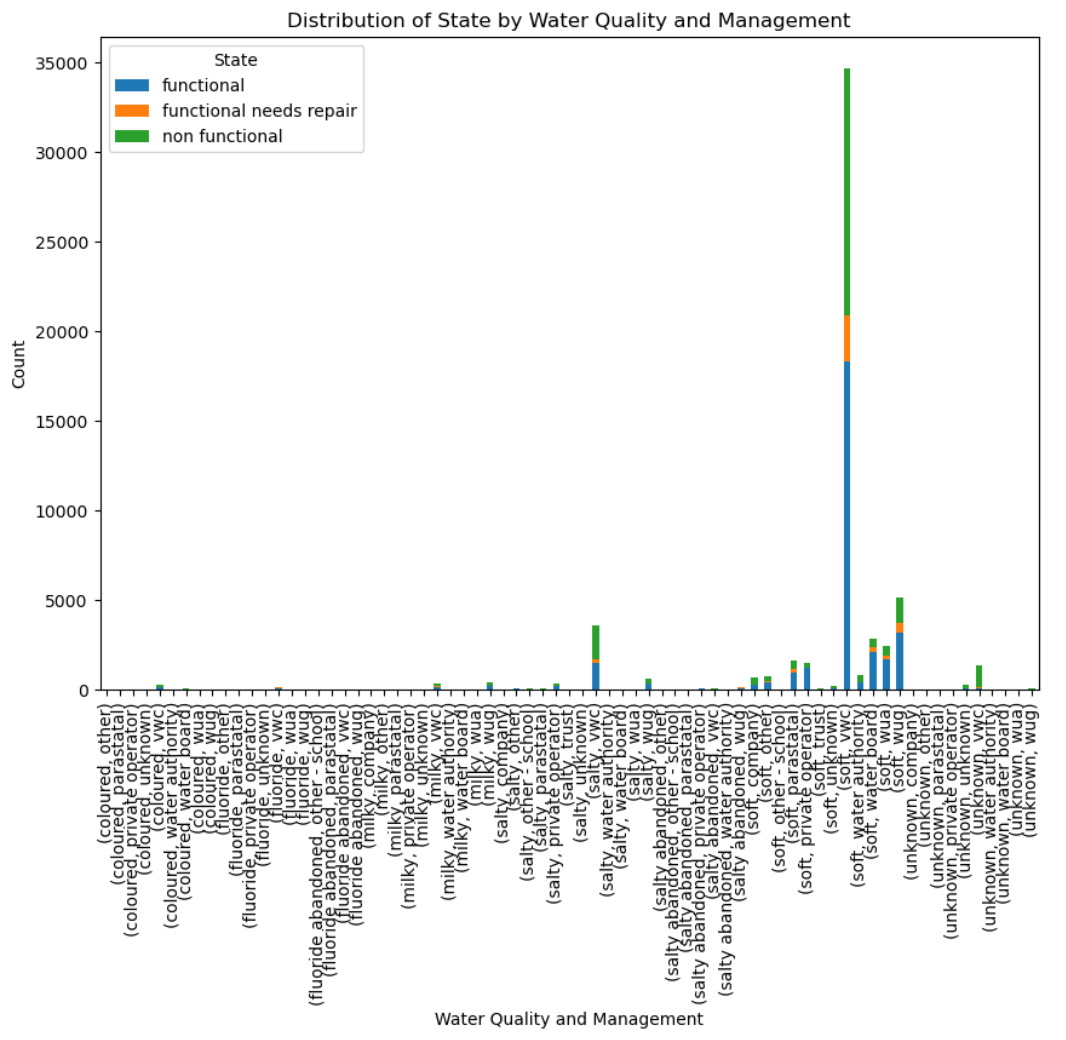
\includegraphics[width=0.5\textwidth]{10.pic.jpg}}
\caption{Distribution of state by water quality and management}
\end{figure}
    
In addition, we also want to analyze the correlation between the features with NaN values and the target features. Since there are so many categories, we first use feature engineering to reduce the number of categories before performing data analysis. Take the three characteristics of funders, installers and scheme managements as examples.

\begin{figure}[H]
\centerline{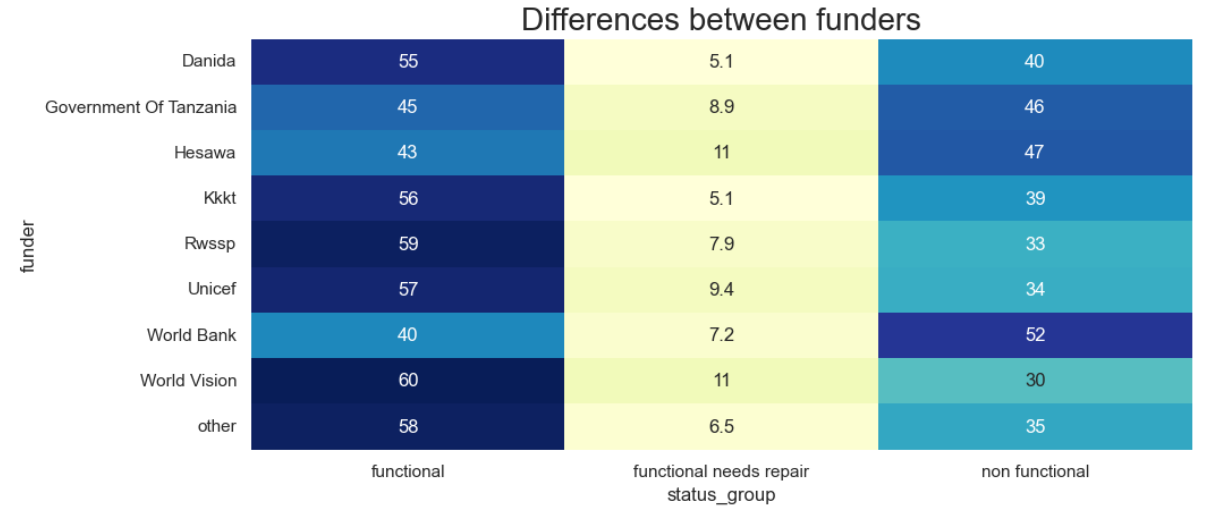
\includegraphics[width=0.5\textwidth]{7.pic.jpg}}
\caption{Differences between funders}
\end{figure}

As shown in Fig. 9, after reducing the number of categories, the state data distribution of different funders to water pumps can be displayed very well. Darker colors represent more distribution.

\begin{figure}[H]
\centerline{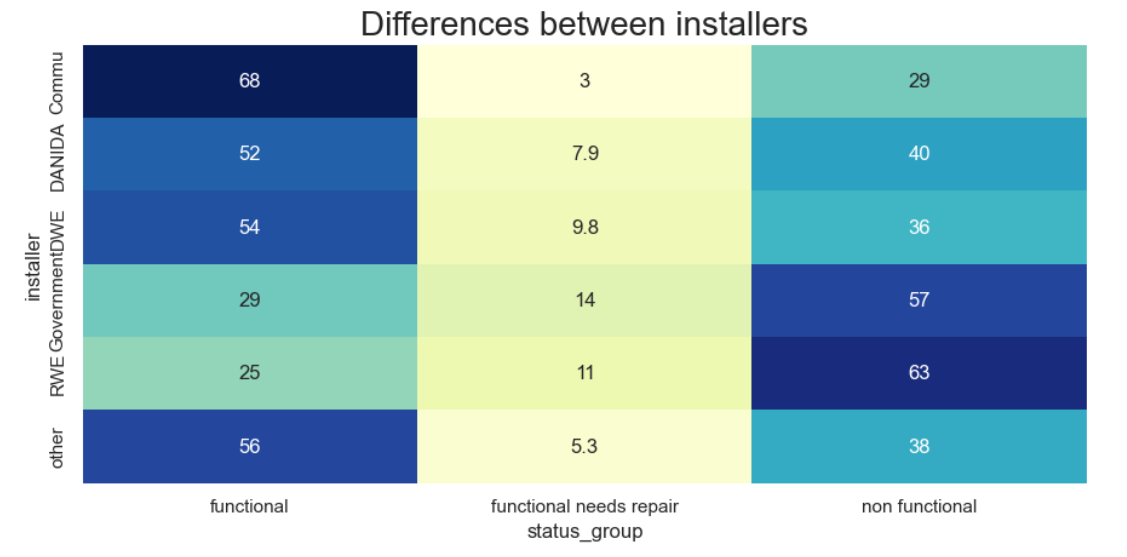
\includegraphics[width=0.5\textwidth]{8.pic.jpg}}
\caption{Differences between installers}
\end{figure}
    
\begin{figure}[H]
\centerline{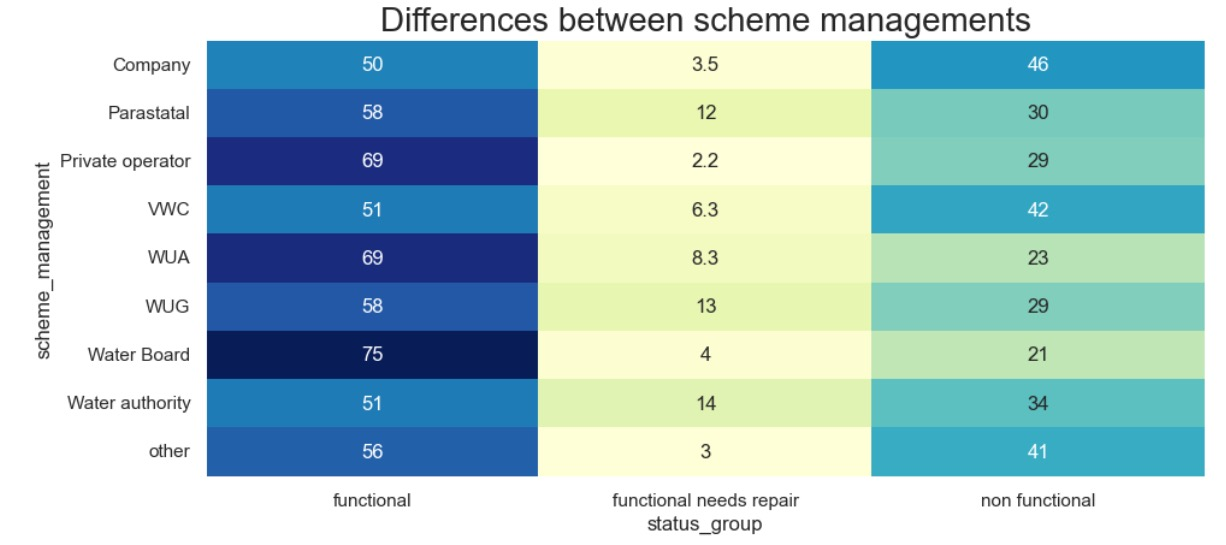
\includegraphics[width=0.5\textwidth]{9.pic.jpg}}
\caption{Differences between scheme managements}
\end{figure}

Similarly, Fig. 10 and Fig. 11 also show the data distribution of installers and scheme managements in the three states of water pumps, such as 'RWE', which is more related to water pumps that cannot work, and 'Water authority', a management organization that can the water pump used is more relevant.

What needs to be added is that although we have used two methods of data analysis, we can notice that descriptive statistical analysis will focus more on the information of the data itself, which is an effective method for basic information collection, while data visualization is more targeted , which can better reflect the relationship between data and is very flexible.

Therefore, in summary, we finally chose to use these two methods for data analysis at the same time, which can help us to find problems in the original data set while analyzing data relationships and laws, and prepare for subsequent data preprocessing.

\subsection{Data pre-processing}

Although some data preprocessing methods have appeared in data analysis, they are only a small part, so this section will introduce the schemes we use in data preprocessing in detail. We tried a total of 4 categories of data preprocessing methods, including data cleaning, data dimensionality reduction, data balancing, and category reduction. These four types of feature engineering methods. Among them, data cleaning includes methods such as missing value processing, feature selection and feature encoding. Data imbalance includes two methods: SMOTE and RandomOverSampler. Data dimensionality reduction uses principal component analysis(PCA), and category reduction uses new classification.

\subsubsection{Category reduction}

Category reduction is generally used to deal with categorical data, especially when dealing with features with a large number of unique classes. It reduces the complexity of this feature, reduces the risk of overfitting, and is easy to visualize and analyze, making the data less sparse. This method was mentioned in the previous data analysis, which is used to study the relationship between some feature columns containing NaN values and the target features. Taking the analysis of 'installers' and water pump status as an example, we found that there are many categories with a count of 1, so we classify the categories with a count of less than 1000 into one category and name them as others. As shown in Fig. 12, this is the data distribution after category reduction processing, which is very clear and solves the problem of data sparseness.

\begin{figure}[H]
\centerline{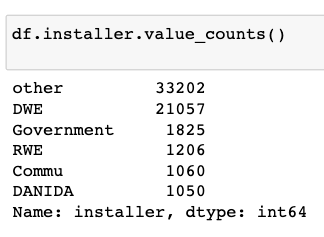
\includegraphics[width=0.3\textwidth]{11.pic.jpg}}
\caption{The result of category reduction for 'installer'}
\end{figure}
    
\subsubsection{Data cleaning}

Because there will always be some errors, duplicates, inconsistencies, or incomplete data in the data set, data cleaning can improve the quality of the data set and improve the performance of subsequent model training. Here, we tried and adopted three methods of missing value handling, feature selection, and feature encoding.

\begin{itemize}
\item \textbf{Missing value handling}

Generally, missing data processing methods include deletion, filling, interpolation, etc. We used the filling method in this data set to process missing data. By statistically calculating the content of the feature column with missing data, we can obtain the mode of the feature column, and use the mode to fill the missing data. As shown in Fig. 13, after the mode filling, the number of all missing values in the data set is 0.

\begin{figure}[H]
\centerline{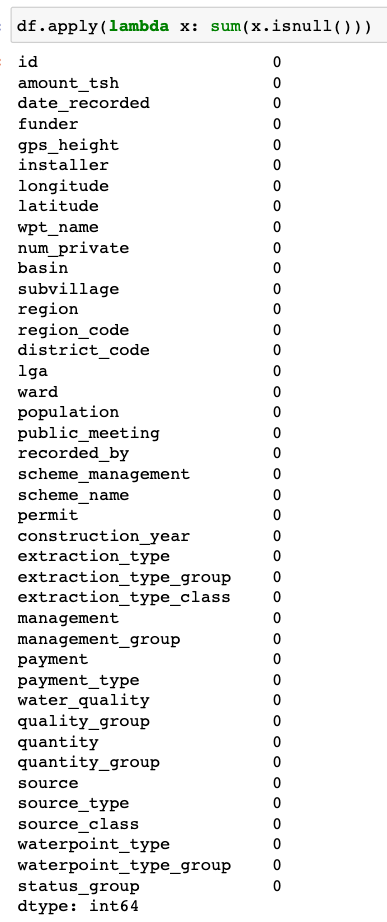
\includegraphics[width=0.2\textwidth]{12.pic.jpg}}
\caption{The result of missing value handling}
\end{figure}
    

\item \textbf{Feature selection}

Feature selection is a relatively important data processing step and a key step in machine learning. It can effectively reduce training time and improve interpretability and model performance. Generally, it can be performed by embedding or filtering methods. In this data set, in order to reduce the complexity, we adopted a relatively simple method. First, we used artificial screening to delete all the feature columns with the same value, and then analyzed some feature columns that were processed by category reduction, and deleted the feature columns that were consistent with the target Feature columns with little correlation between features. In addition, we also remove some duplicate feature columns and meaningless feature columns from the dataset. As shown in Fig. 14, these are the feature names left after feature selection.

\begin{figure}[H]
\centerline{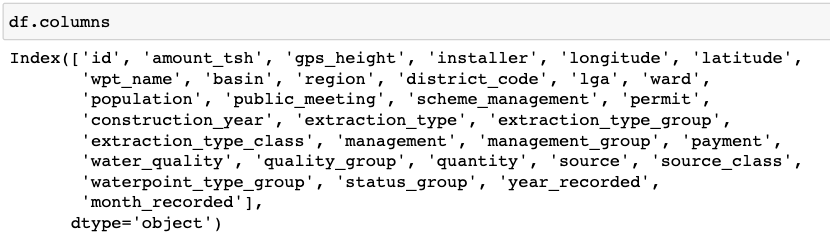
\includegraphics[width=0.5\textwidth]{13.pic.jpg}}
\caption{The result of missing feature selection}
\end{figure}
    
\item \textbf{Feature encoding}

By observing the data set after data filling and feature selection, we can find that the format of most feature data is object. In order to facilitate subsequent data classification and model training, we need to use feature encoding to convert the classified data into a format that can be used in machine learning algorithms. Common feature encoding methods include label encoding, one-hot encoding, target encoding, etc. Here, we use label encoding. It can map each category to an integer, for example, 'functional' corresponds to 2, 'functional needs repair': corresponds to 1, 'non functional' corresponds to 0. As shown in Figure 15, it shows the result of label encoding for a column of categorical data.

\begin{figure}[H]
\centerline{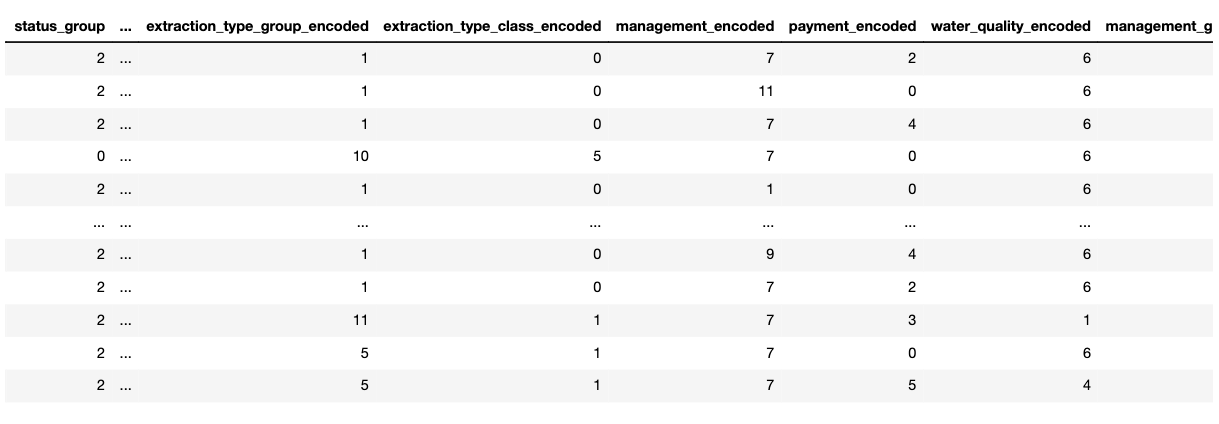
\includegraphics[width=0.5\textwidth]{14.pic.jpg}}
\caption{The result of feature encoding}
\end{figure}
\end{itemize}

\subsubsection{Data dimensionality reduction}

Although feature selection has screened out part of the data, there are still many problems in the high-dimensional feature space. Therefore, in order to solve this potential risk, data dimensionality reduction is a more effective method. It can convert high-dimensional feature space into low-dimensional feature space, reduce computational complexity, and allow us to better understand the structure of the data. Common data dimensionality reduction techniques include principal component analysis (PCA) and linear discriminant analysis (LDA). Here, we use PCA for data dimension reduction, which transforms the original data into a set of linearly independent representations of each dimension through linear transformation, which can be used to extract the main feature components of the data. As shown in Fig. 16, it shows the result of transforming the raw data into 20 feature columns.

\begin{figure}[H]
\centerline{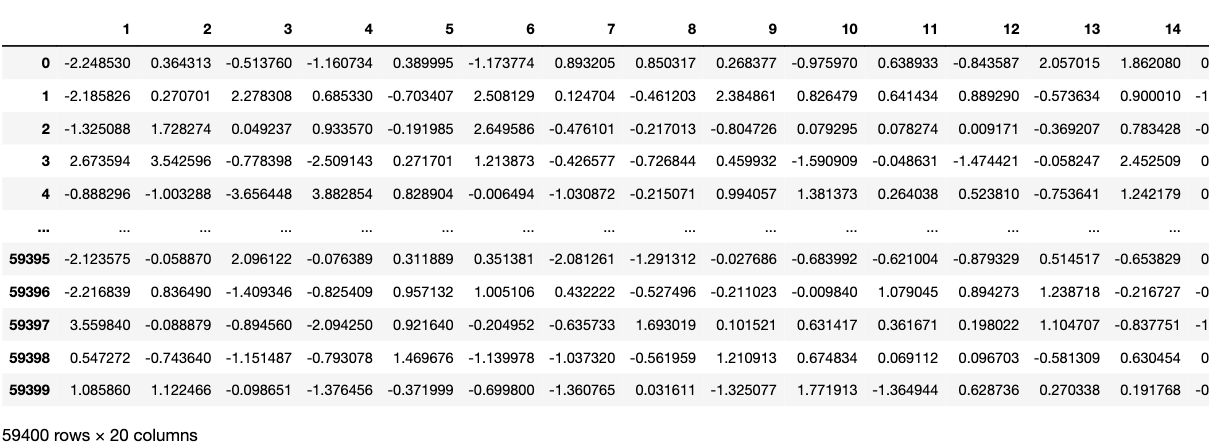
\includegraphics[width=0.5\textwidth]{15.pic.jpg}}
\caption{The result of PCA}
\end{figure}
    
\subsubsection{Data imbalance}

In the above data analysis, by observing Fig. 5, we can find that the number of 'functional needs repair' of the target feature is significantly less than that of the other two feature classes, and the gap is very wide, which often leads to a significant decline in the performance of machine learning. And it will be biased towards the category with a large number of predictions. In order to solve this hidden danger, we need to use some strategies, such as oversampling, undersampling, modifying performance indicators, etc. Here, we tried two methods for data imbalance processing, they are SMOTE and RandomOverSampler.

\begin{itemize}
\item \textbf{SMOTE}

SMOTE is a kind of oversampling technology. Its basic idea is to generate new minority class samples by interpolating minority class samples, and increase the number of minority class samples to achieve class balance. It is generally implemented in two steps. First, for each minority class sample, calculate the distance between it and other minority class samples, and find its k nearest neighbor samples, and then select one of them according to the set oversampling ratio or Multiple nearest neighbor samples, and then for each selected nearest neighbor sample, randomly select a point on the connection line between it and the original sample as a newly generated minority class sample \cite{b5}.

\begin{figure}[H]
\centerline{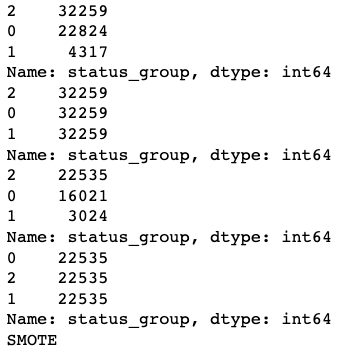
\includegraphics[width=0.3\textwidth]{16.pic.jpg}}
\caption{The result of SMOTE}
\end{figure}

As shown in Fig. 17, it shows the number of different classes of target features after SMOTE processing on the training set. Obviously, the numbers of the three classes are all filled to the same number.

\item \textbf{RandomOverSampler}

RandomOverSampler is also a kind of oversampling, which increases the number of samples by randomly copying the samples of the minority class, so as to achieve class balance. As shown in Fig. 18, it shows the results of data imbalance processing using RandomOverSampler, and the number of completions for each category is the same as the previous method.

\begin{figure}[H]
\centerline{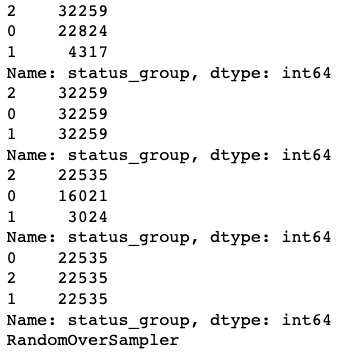
\includegraphics[width=0.3\textwidth]{17.pic.jpg}}
\caption{The result of RandomOverSampler}
\end{figure}

It should be noted that random oversampling may increase the risk of overfitting of the model, because it increases the number of minority class samples by duplicating them, which may cause the model to be overly sensitive to these duplicated samples\cite{b6}. Therefore, this data set does not consider the use of RandomOverSampler for data imbalance processing.
\end{itemize}

So far, all the data preprocessing methods we have tried have been introduced. Because they need to be divided into two groups for comparison, we will divide the above data preprocessing methods into two categories. The first category includes category reduction, data cleaning and Data dimensionality reduction (PCA), the second category includes category reduction, data cleaning and data balancing (SMOTE). Due to the relationship of the original data set, both methods need to include category reduction and data cleaning.

What needs to be added is that for the accuracy of the model, we finally integrated and used four steps of category reduction, data cleaning, data dimensionality reduction (PCA) and data balance (SMOTE) to preprocess the data, and obtained the highest prediction accuracy.

\subsection{Data classification}

In order to classify and predict the preprocessed dataset, we need to select an appropriate model for training and performance evaluation. Here, we have selected two popular models for training, they are DecisionTree and XGBoost, which just correspond to the training set after the preprocessing of the previously divided two types of data, and then carry out model training and evaluation.

\subsubsection{DecisionTree}

For the model training of the DecisionTree, we choose the first type of preprocessed data set, that is, the data set processed by category reduction, data cleaning and Data dimensionality reduction (PCA).

\begin{figure}[H]
\centerline{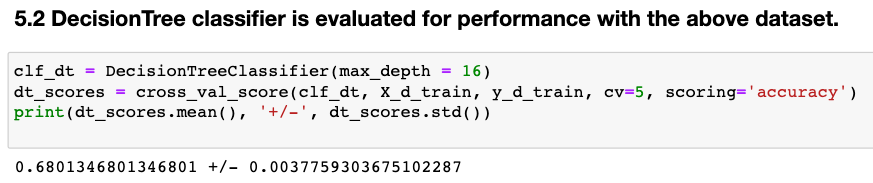
\includegraphics[width=0.5\textwidth]{18.pic.jpg}}
\caption{Accuracy of DecisionTree in the first type of preprocessed data set}
\end{figure}

As shown in Fig. 19, the accuracy rate of the model is about 68\%, which is not high.

\subsubsection{XGBoost}

For the model training of the XGBoost, we choose the second type of preprocessed data set, that is, the data set processed by category reduction, data cleaning and data balancing (SMOTE).

\begin{figure}[H]
\centerline{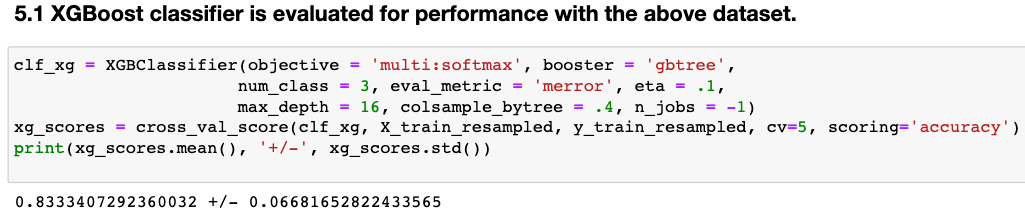
\includegraphics[width=0.5\textwidth]{19.pic.jpg}}
\caption{Accuracy of decision tree in the second type of preprocessed data set}
\end{figure}

As shown in Fig. 20, the accuracy rate of this model is about 83.3\%, which is relatively high.

In addition, in order to have a high accuracy rate, we have gone through various data preprocessing and model combinations and tests, and finally found the best performance match. The data preprocessing includes category reduction, data cleaning, data dimensionality reduction (PCA)
and data balance (SMOTE) four steps, the model finally chose XGBoost.

\begin{figure}[H]
\centerline{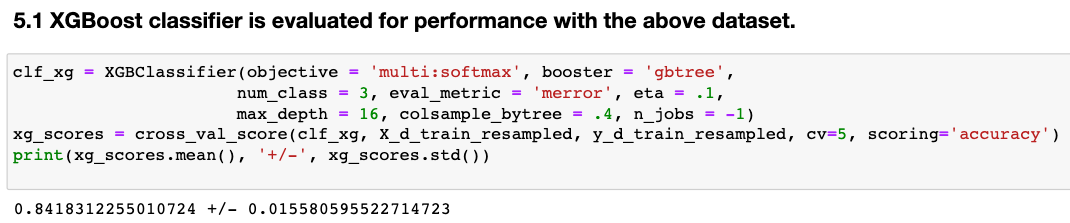
\includegraphics[width=0.5\textwidth]{20.pic.jpg}}
\caption{Final accuracy}
\end{figure}
    
As shown in Fig. 21, the final accuracy of the model is as high as 84.1\%.

\begin{figure}[H]
\centerline{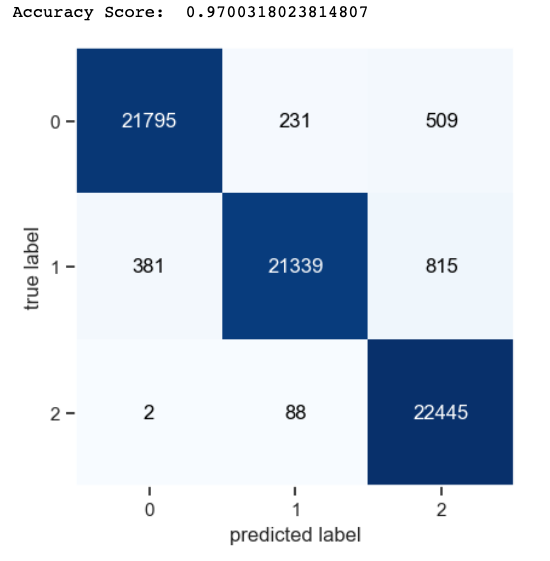
\includegraphics[width=0.4\textwidth]{21.pic.jpg}}
\caption{Confusion matrix image}
\end{figure}
    
Fig. 22 shows the performance of the model on the oversampled training dataset after training with appropriate XGBoost parameters. It can be seen that the accuracy rate is very high.

Finally, we applied the model to the test data set, and the final classification prediction results are shown in Fig. 23.

\begin{figure}[H]
\centerline{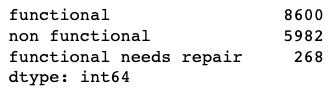
\includegraphics[width=0.3\textwidth]{22.pic.jpg}}
\caption{Prediction on test set}
\end{figure}

\section{Discussion}
\subsection{Comparing and critiquing (partners in pair)}

As mentioned above, the first solution is to use the first type of preprocessed data set to train the DecisionTree model, and its final accuracy rate is 68\%; the second solution is to use the second type of preprocessed data set to train XGBoost model, its final accuracy rate is 83.3\%.

Obviously, the accuracy rate of option 1 is very low, and the accuracy rate of option 2 is higher. The reason for the low accuracy of Scheme 1 may be that the DecisionTree model itself has poor performance in this data set, and data imbalance and PCA have negatively affected the data set. Although the accuracy of Scheme 2 is higher, there are still cases of overfitting after data imbalance processing, and the feature dimension is high, and the calculation is complicated and takes a long time.

\subsection{Comparing and critiquing (previous research)}

In this section, we use the scheme with the highest final accuracy for comparison with previous studies.

Darmatasia and Aniati also used XGBoost to create a model in their study, but the accuracy of their model was only 80.38\%, lower than our experimental result of 84\%, which may be because they did not consider the imbalance of the categories of data sets when processing the data. This may lead to overfitting problems and deviations in the predicted results of the model\cite{b1}.

Karan and L's TabNet model also obtained good prediction results, with an accuracy of 83.6\%, which may be attributed to their substitution strategies for some columns with category skew. TabNet can also learn nonlinearities in the data and avoid the problem of over-fitting. At the same time, TabNet uses sequential attention to select prominent features in each decision step, which contributes to the interpretability of the model, which is not involved in our study\cite{b2}.

In Jacob's study, a random forest model with an accuracy of 82.09\% was created. During the study, he conducted correlation assessment for each single feature, and conducted correlation statistics by chi-square test or analysis of variance test according to the type of variable. This is quite sufficient for the data analysis and selection, to ensure the reliability of the data, for the training model is very helpful. At the same time, this is what we need to improve in our research work\cite{b3}.

Among the models created by Indra and Vivek, the one that achieved the best results was also the RandomForest model, but neither the accuracy of the model nor the specific data processing process were given, so there may be insufficient data processing, so the trained model is not reliable and persuasive enough\cite{b4}.

\section{Conclusions and recommendation for future research}

This study uses appropriate data analysis, data preprocessing, and data classification methods to process and select features to ensure the integrity and reliability of the data set, and selects the most relevant features to construct prediction models, thereby ensuring that the trained models can obtain reliable results during prediction.

We use different data mining techniques to construct models to predict the operating status of water supply points, using methods such as Decision tree and XGBoost. In addition, the performance of two different models was compared, such as the time required for training and the accuracy of prediction results. The final experimental results indicate that the prediction accuracy of the XGBoost model is higher than that of the decision tree.

In addition, we also compared and analyzed the impact of natural factors (such as water quality, water source types, geographical location) and human factors (such as management, management level) on the status of waterpoints, to understand the impact of these two factors on water supply point conditions, and provide important reference information for decision-makers to improve the effect of water supply management and maintenance and operation.

In summary, both of the prediction models we have constructed can predict the state of water pumps, but the XGBoost model has better performance and higher accuracy. Our analysis of data can also provide managers with some reference information, allowing them to understand which factors have a significant impact on the status of water pumps, and to pay more attention in future maintenance and management.

\begin{thebibliography}{00}
\bibitem{b1} Arymurthy, A.M., 2016, October. Predicting the status of water pumps using data mining approach. In 2016 International Workshop on Big Data and Information Security (IWBIS) (pp. 57-64). IEEE.
\bibitem{b2} Pathak, K. and Shalini, L., 2023. Pump It Up: Predict Water Pump Status using Attentive Tabular Learning. arXiv preprint arXiv:2304.03969.
\bibitem{b3} Benoot, J., PREDICTING THE FUNCTIONAL STATE OF TANZANIAN WATER PUMPS.
\bibitem{b4} Chowdavarapu, I.K. and Manikandan, V.D., 2016. Data Mining the Water Pumps: Determining the functionality of Water Pumps in Tanzania using SAS Enterprise Miner. SAS South Central User Group Forum.
\bibitem{b5} Chawla, N. V., Bowyer, K. W., Hall, L. O., \& Kegelmeyer, W. P. (2002). SMOTE: Synthetic Minority Over-sampling Technique. Journal of Artificial Intelligence Research, 16, 321-357.
\bibitem{b6} Lemaitre, G., Nogueira, F., \& Aridas, C. K. (2017). Imbalanced-learn: A Python Toolbox to Tackle the Curse of Imbalanced Datasets in Machine Learning. Journal of Machine Learning Research, 18(17), 1-5.
\end{thebibliography}

\end{document}
